\documentclass{ikpKoeln}
\usepackage{graphicx}
\usepackage{physics}
\usepackage{xcolor}
\usepackage[skip=0pt]{caption}
\usepackage{tikz}
\usepackage{siunitx}
\usetikzlibrary{math}
\usepackage[listings,theorems]{tcolorbox}
\usepackage{tabularray}

\scTitle{Application of the Millepede II algorithm to the NeuLAND time-position calibration}
\scAuthor{*}{Yanzhao}{Wang}{1}
\scAuthor{}{Luca}{Flandoli}{1}
\scAuthor{}{Igor}{Gasparic}{2}
\scAuthor{}{Andreas}{Zilges}{1}
\scAffiliation{1}{University of Cologne, Institute for Nuclear Physics, Germany}
\scAffiliation{2}{GSI Helmholtzzentrum für Schwerionenforschung, Germany}
\scEmail{ywang@ikp.uni-koeln.de}

\scTitleShort{Millepede algorithm for the NeuLAND Calibration}

\date{\scriptsize T 56.4\\DPG-Frühjahrstagung\\Erlangen 2026 \\ \vspace{1em} Supported by BMBF (05P24PK1)}

\graphicspath{{../figures/}}

\DeclareSourcemap
{
    \maps[datatype=bibtex,overwrite=true]
    {
        \map{
        \step[fieldsource=journal,
           match={Nuclear Instruments and Methods in Physics Research, Section A: Accelerators, Spectrometers, Detectors, and Associated Equipment},
           replace={Nucl. Instrum. Methods Phys. Res., Sect. A}]
            }
    }
}

\addbibresource{reference.bib}

\newlength{\myeqskip}
\setlength{\myeqskip}{3pt}

\AtBeginDocument{%
    \setlength\abovedisplayskip{\myeqskip}%
    \setlength\belowdisplayskip{\myeqskip}%
    \setlength\abovedisplayshortskip{\dimexpr\myeqskip-\baselineskip\relax}%
    % \setlength\abovedisplayshortskip{\baselineskip }%
    \setlength\belowdisplayshortskip{\myeqskip}
}
\AtBeginEnvironment{frame}{\setcounter{footnote}{0}}

% \AtBeginDocument{\RenewCommandCopy\qty\SI}

\newtcolorbox{graybox}{%
    colframe=gray,
    sharp corners=all,
    top=0mm,
    left=0mm,
    bottom=0mm,
    leftright skip=-1mm,%
}

\definecolor{TitleBoxBackColor}{RGB}{219, 228, 241}
\definecolor{TitleBoxBorderColor}{RGB}{23, 54, 93}

\newtcolorbox{titlebox}[2][]{%
    sharp corners=all,
    left=0mm,
    top=0mm,
    bottom=0mm,
    leftright skip=-1mm,%
    colframe=TitleBoxBorderColor,
    colback=TitleBoxBackColor,
    coltitle=black,
    title={#2},
    fonttitle=\bfseries,
    detach title,before upper={\tcbtitle\par},
    #1,
}


\begin{document}

\titleFrame

{
	\usebackgroundtemplate{%
		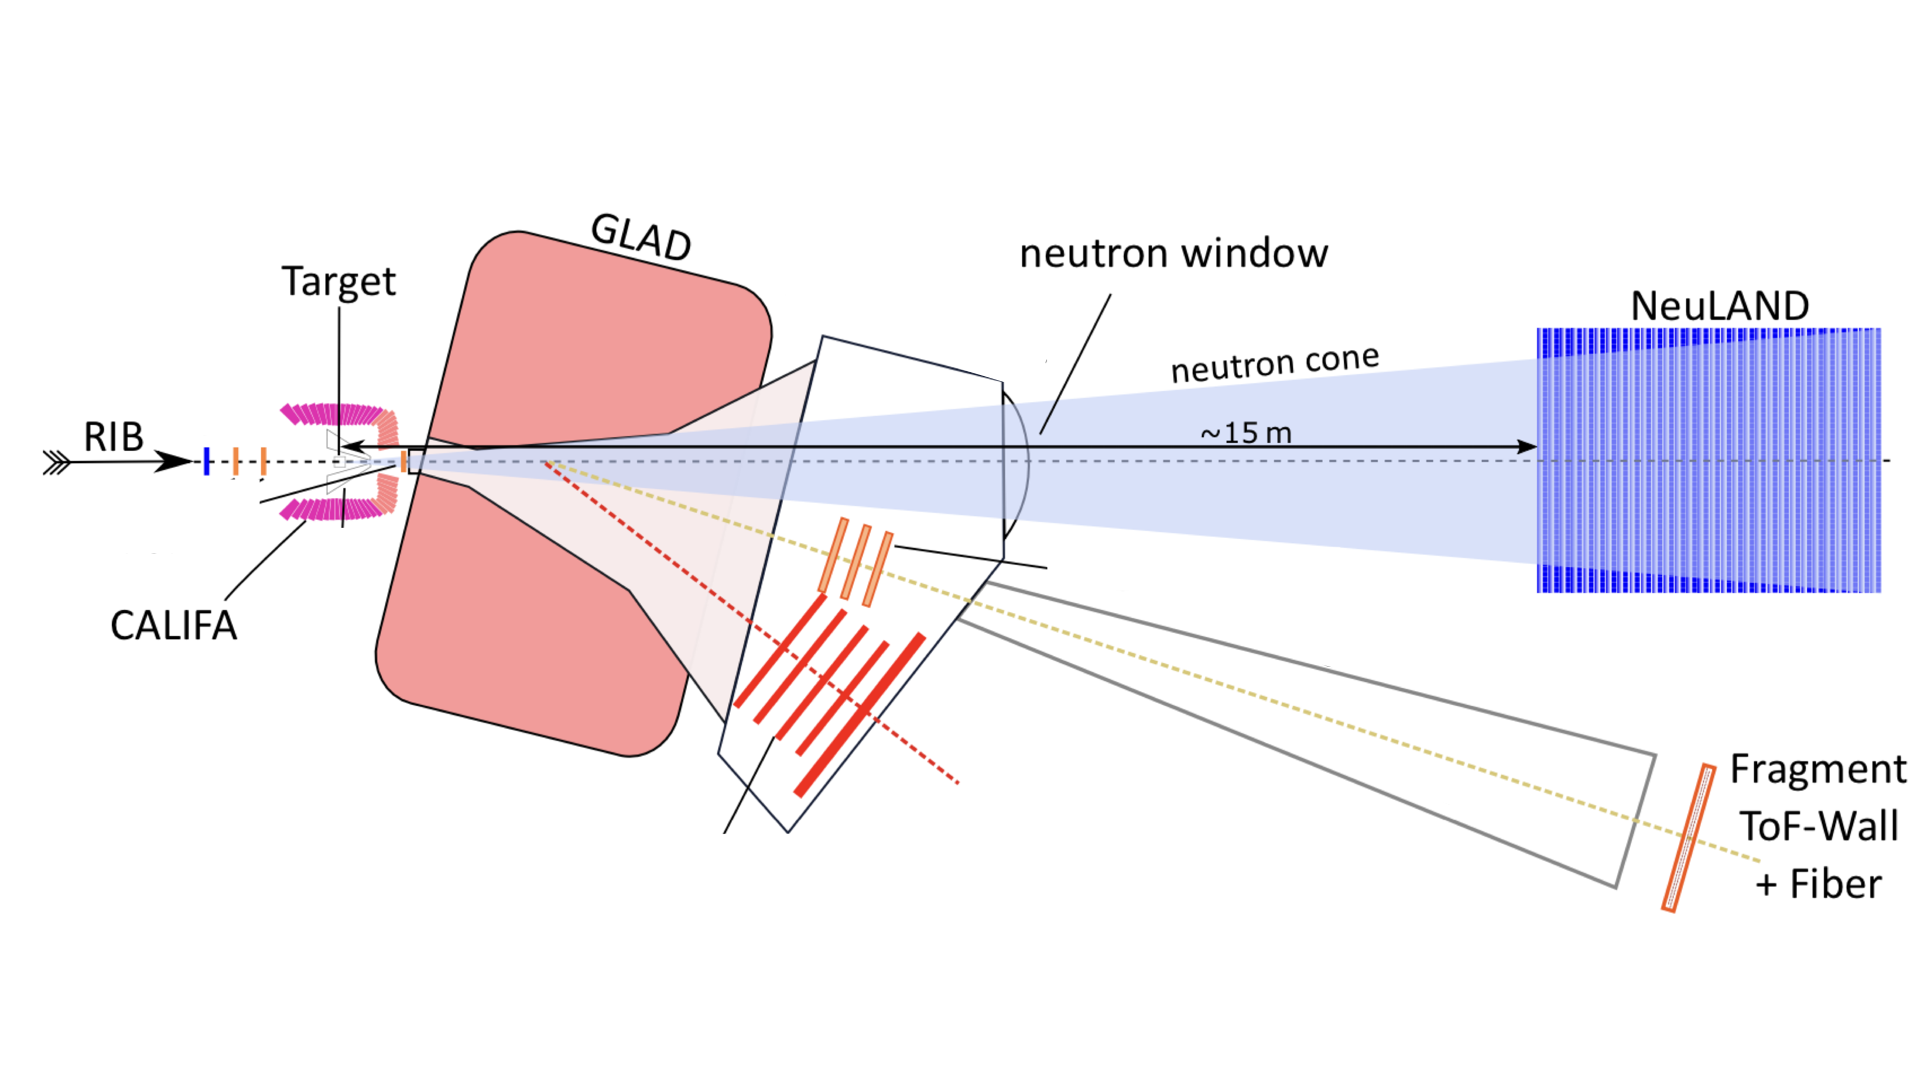
\includegraphics[width=\paperwidth, height=\paperheight]{r3b/r3bsetup_empty.png}}
	\begin{frame}{NeuLAND setup in $\text{R}^3\text{B}$ at FAIR\footfullcite{BORETZKY}}

		\begin{columns}[c]
			\begin{column}{0.4\textwidth}
				\pause
				\begin{figure}
					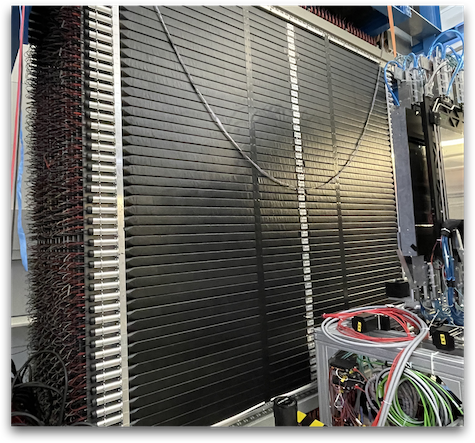
\includegraphics[width = \textwidth]{neuland/neulandReal}
				\end{figure}
			\end{column}
			\hspace*{0.5cm}
			\begin{column}{0.3\textwidth}
				\begin{exampleblock}{}
					Geometry:\\
					\begin{itemize}
						\item $26$ planes
						\item $\qtyproduct[product-units=power]{250 x 250}{\centi\meter}$
						\item $50$ scintillators each plane
						\item $1300$ Bars in total
						\item $2600$ PMTs in total
					\end{itemize}
					Output:\\
					\begin{itemize}
						\item Time values
						\item Positions
					\end{itemize}
				\end{exampleblock}
			\end{column}
			\begin{column}{0.3\textwidth}
			\end{column}
		\end{columns}
		% \let\thefootnote\relax\footnotetext{\fullcite{BORETZKY}}
	\end{frame}
}

\begin{frame}[t]{NeuLAND time and position calibration}
	\vspace*{-1em}
	\begin{columns}[t]
		\begin{column}{0.4\textwidth}
			\textbf{Calibration with cosmic muons}:
			\begin{figure}
				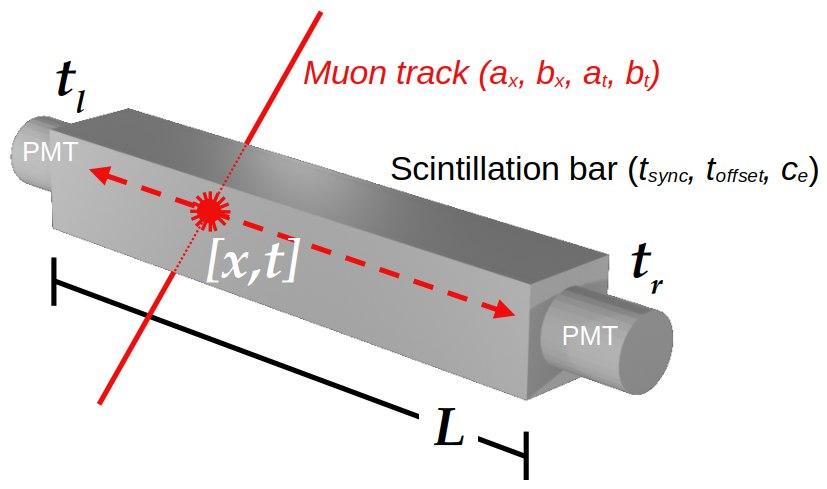
\includegraphics[width=\textwidth]{DPG2026/NeulandBar}
				\caption*{
					\alert{3900} parameters from scintillators and \alert{$6N$} parameters from $N$ muon tracks
				}
			\end{figure}
		\end{column}
		\begin{column}{0.45\textwidth}
			\pause
			\textbf{Current method}:
			using active bar positions to reconstruct muon tracks:
			\begin{figure}
				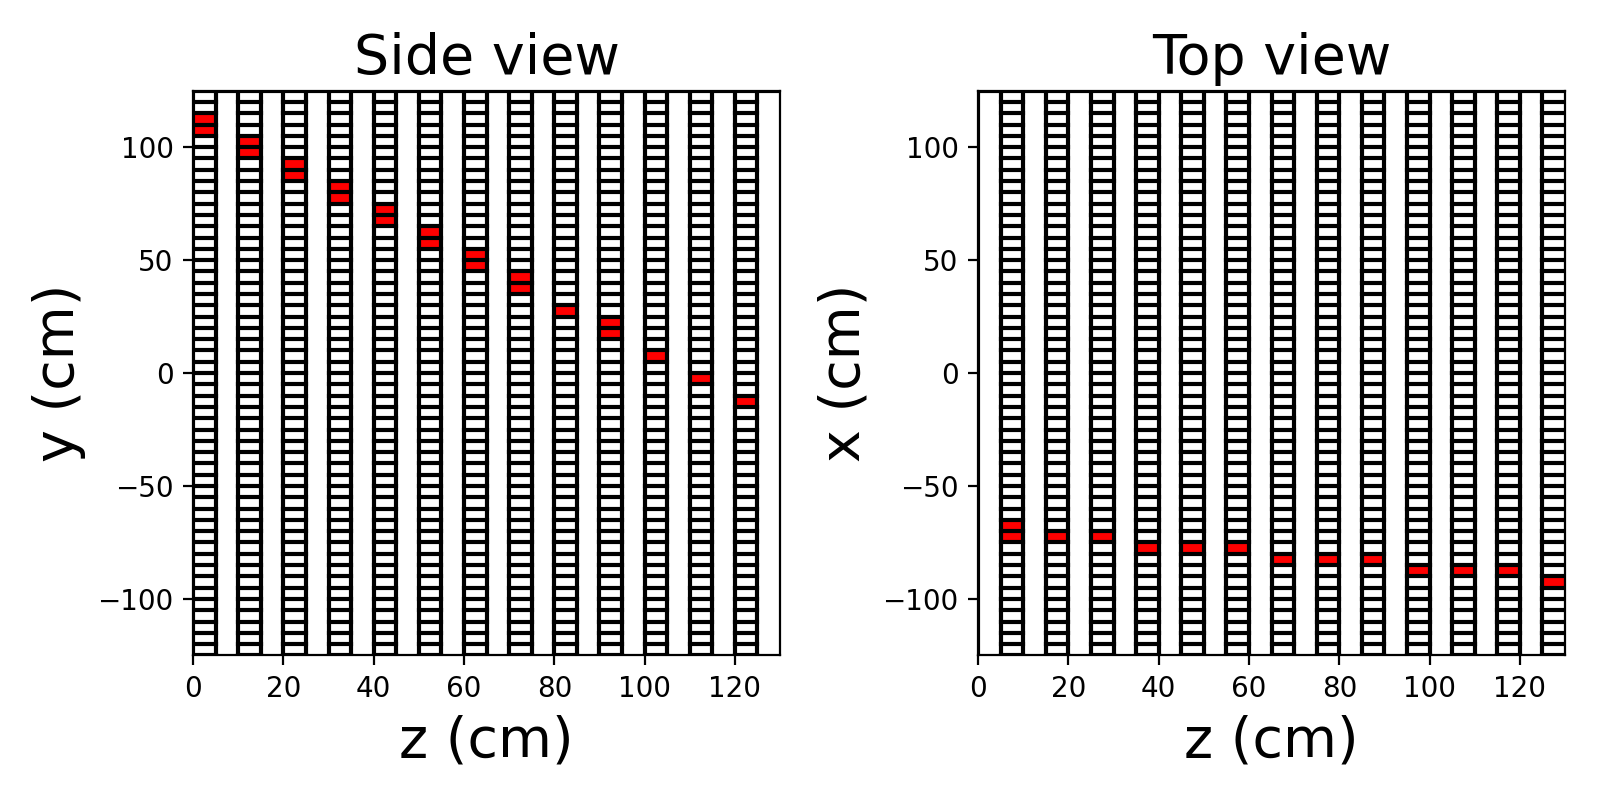
\includegraphics[width=\textwidth]{DPG2026/BarPositions}
			\end{figure}
		\end{column}
	\end{columns}
	\vspace*{-1em}
	\begin{columns}[t]
		\begin{column}{0.4 \textwidth}
			\begin{exampleblock}{Calibration relations}
				\vspace{-1em}
				\begin{align}
					\alert{b_x} + z \cdot \alert{a_x} + \alert{c_e} \cdot t_\text{diff} /2 - \alert{t_\text{offset}}/2                  & = 0 \\
					\alert{b_t} + z \cdot \alert{a_t} + \alert{t_\text{sync}} + \frac{\mathcal{L}}{2\cdot \alert{c_e}} - t_\text{sum}/2 & = 0
				\end{align}
			\end{exampleblock}
		\end{column}
		\begin{column}{0.45 \textwidth}
			\begin{block}{Relations with known muon tracks}
				\vspace{-1em}
				\begin{align}
					\mathcal{C}(a_x, b_x, z) + \alert{c_e} \cdot t_\text{diff} - \alert{t_\text{offset} }                                    & = 0 \\
					\mathcal{C}(a_t, b_t, z, t_\text{sum}) \cdot \alert{c_e} + 2 \cdot \alert{t_\text{sync}} \cdot \alert{c_e} + \mathcal{L} & = 0
				\end{align}

			\end{block}
		\end{column}
	\end{columns}
\end{frame}

\begin{frame}[t]{Minimization with Newton's method}
	\vspace{-1em}
	\begin{columns}[t]
		\begin{column}{0.5\textwidth}
			\vspace{-2em}
			\begin{titlebox}{Objective function minimization}
				$$\vec{P}, \vec{Q} = \operatorname*{argmin}_{\vec{p}, \vec{q}} f(\vec{p}, \vec{q}, z, t_\text{diff}, t_\text{sum})$$
				{
						\textit{where}
						\begin{flalign*}
							\setlength{\belowdisplayskip}{0pt}
							\setlength{\abovedisplayskip}{0pt}
							\hspace{3mm} \vec{p} & : \text{Parameters of scintillators}                                                   & \\
							\vec{q}              & : \text{Parameters of all muon tracks }(\vec{q}^0, \ \vec{q}^1, \ \ldots, \ \vec{q}^N) &
						\end{flalign*}
					}
			\end{titlebox}
		\end{column}
		\begin{column}{0.45\textwidth}
			\onslide<2->
			{
				\textbf{Newton's method}
				\begin{figure}
					% https://suzyahyah.github.io/calculus/optimization/2018/04/06/Taylor-Series-Newtons-Method.html
					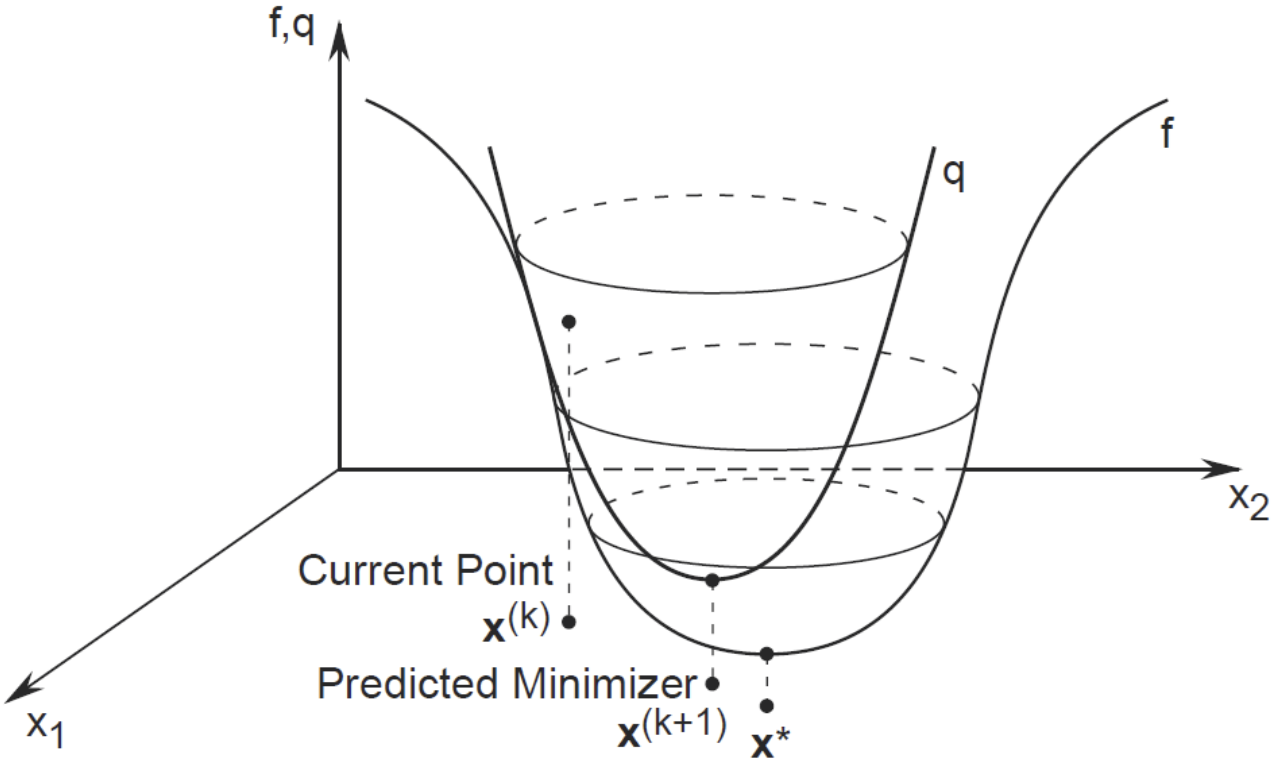
\includegraphics[width=0.7\textwidth]{DPG2026/NewtonsMethod}
				\end{figure}
			}
		\end{column}
	\end{columns}
	\begin{columns}[t]
		\begin{column}{0.5 \textwidth}
			\onslide<3->
			{
				\begin{alertblock}{Limitations of Newton's method}
					\begin{itemize}
						\item Evaluation of Hessian is very expensive. (Quasi Newton's methods, e.g. BFGS)
						\item Expensive computation with a very large number of parameters.
					\end{itemize}
				\end{alertblock}
				Dimension of $\alert{\mathcal{B}(\vec{w})}$ when using N muon tracks:
				$$3900 + 6N \sim \mathcal{O}(N)$$
			}
		\end{column}
		\begin{column}{0.45 \textwidth}
			\onslide<2->
			{
				\begin{graybox}
					\textbf{$n^\text{th}$ iteration for all parameters}
					\begin{flalign*}
						 &                                     & \overrightarrow{W}_{n+1} & = \overrightarrow{W}_{n} - \eta \cdot \left.  \alert{\mathcal{B}(\vec{w})^{-1}} \nabla f(\vec{w}) \right|_{\vec{w} = \overrightarrow{W}_{n}} \hspace{-8em} &                         & \\
						 & \textit{\small where} \hspace{-2em} &                          &                                                                                                                                                            &                           \\
						 &                                     & \vec{w}                  & = \left(\vec{p}, \ \vec{q}^0, \ \vec{q}^1, \ \ldots, \ \vec{q}^N \right)  \hspace{-2em}                                                                    &                         & \\
						 &                                     & \eta                     & = 1                                                                                                                                                        & \text{(Line search)}    & \\
						 &                                     & \mathcal{B}(\vec{w})     & = \nabla^2 f(\vec{w})                                                                                                                                      & \text{(Hessian matrix)} &
					\end{flalign*}

				\end{graybox}
			}
		\end{column}
	\end{columns}
\end{frame}


\begin{frame}[t]{Minimization with Millepede algorithm}
	\vspace{-1em}
	\begin{block}{Parameter properties in calibration with muon tracks}
		\begin{itemize}
			\item Only the result of parameters related to scintillation bars is needed.
			\item Parameters related to one muon track is independent to another.
		\end{itemize}
	\end{block}
	\pause
	Separation into \textbf{global} and \textbf{local} parameters in Millepede algorithm:
	$\begin{tblr} {X[3,c]|[1.5pt]X[2,c]|X[2,c]|X[2,c]} \hline
			\text{Global parameters}\ \vec{p}_i & \text{Local parameters} \ \vec{q}^0      & ... & \text{Local parameters} \ \vec{q}^N      \\ \hline
			p_1, p_2, \ldots, p_{3900}          & a^0_x, b^0_x, a^0_y, b^0_y, a^0_t, b^0_t & ... & a^N_x, b^N_x, a^N_y, b^N_y, a^N_t, b^N_t \\ \hline
		\end{tblr}$

	\vspace{-0.5em}
	\pause
	\begin{columns}[t]
		\begin{column}{0.6 \textwidth}
			\begin{graybox}
				\textbf{$n^\text{th}$ iteration for global parameters\footnotemark}
				\begin{flalign*}
					 &                               & \vec{p}_{n+1}                  & = \vec{p}_{n} - \left.  \mathcal{B}(\vec{p}, \vec{q})^{-1} \left(\nabla_p f + \mathcal{R}(\vec{p}, \vec{q})\nabla_q f \right) \right|_{\vec{p} = \vec{p}_{n}, \vec{q} = \vec{q}^n} \hspace{-7em} &                                          & \\
					 & \textit{where}: \hspace{-7em} &                                &                                                                                                                                                                                                  &                                          & \\
					 &                               & \mathcal{B}(\vec{p}, \vec{q})  & =  \nabla^2_pf  -\nabla^2_{pq}f \cdot \nabla^2_{q}f \cdot \left(\nabla^2_{pq}f\right)^\intercal                                                                                                  & (\text{size: } \alert{3900 \times 3900}) & \\
					 &                               & \mathcal{R} (\vec{p}, \vec{q}) & = - \nabla^2_{pq}f \cdot \left(\nabla^2_qf\right)^{-1}                                                                                                                                           & (\text{size: } \alert{3900 \times 6})    &
				\end{flalign*}
			\end{graybox}
		\end{column}
		\begin{column}{0.35 \textwidth}
			\begin{exampleblock}{Advantages of Millepede algorithm}
				\begin{itemize}
					\item Still simultaneous fitting of all parameters
					\item Computation complexity independent of the number of muon tracks
				\end{itemize}
			\end{exampleblock}
		\end{column}
	\end{columns}
	\footnotetext<3->{For the full derivation, please visit Millepede-II manual (url: \url{https://www.desy.de/~kleinwrt/MP2/doc/html/draftman_page.html})}
\end{frame}

\begin{frame}[t]{Millepede-II program and adaptation to NeuLAND \footnotemark}
	\vspace{-1em}
	\begin{columns}[t]
		\begin{column}{0.45 \textwidth}
			\textbf{Millepede-II program structure}
			\begin{figure}
				\begin{center}
					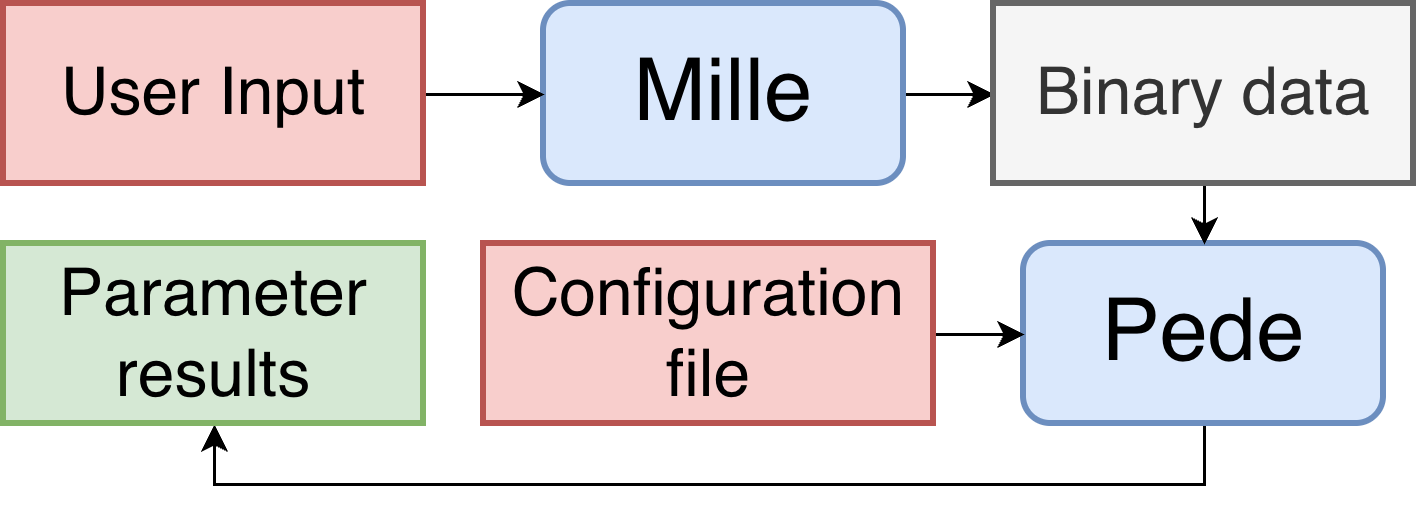
\includegraphics[width=0.95\textwidth]{DPG2026/MillepedeStruct.png}
				\end{center}
			\end{figure}
			\begin{titlebox}{Prerequisites}
				\begin{itemize}
					\item Calibration equation must be \alert{linear}.
					      $$M(z, t) = \sum_{i}G^i(z, t)p^i +\sum_{j}L^j(z, t)q^j $$
					\item "Good" initial global parameter values.
					\item No rank deficit.
				\end{itemize}
			\end{titlebox}
            \footnotetext[1]{\scriptsize Full documentation can be seen via \url{https://yanzhaow.github.io/R3BRoot/neuland_cal.html}}
		\end{column}
		\begin{column}{0.45 \textwidth}
			\pause
			\textbf{Rank deficit in calibration equations}
			\vspace{-2em}
			\begin{figure}
				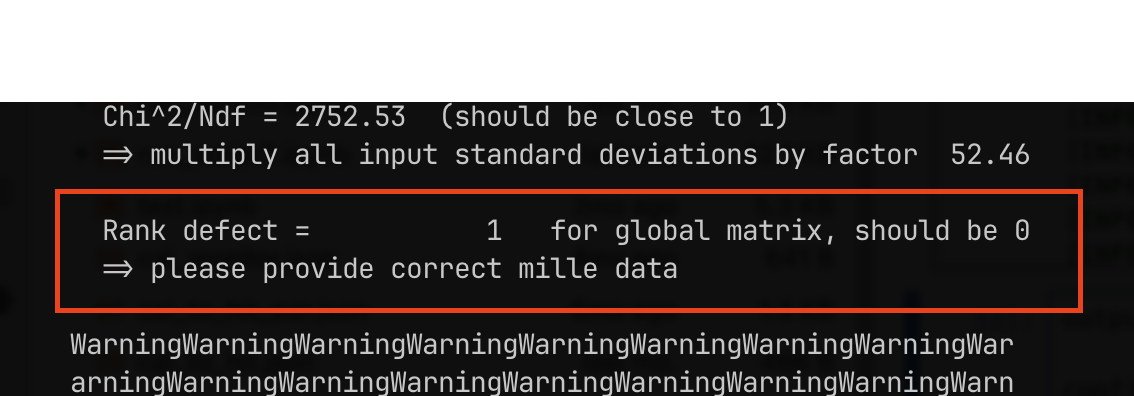
\includegraphics[width=0.8\textwidth]{DPG2026/RankDeficit}
			\end{figure}
			{\footnotesize
			\textbf{A simple example}:
			\begin{equation*}
				\setlength\abovedisplayskip{1mm}
				\setlength\belowdisplayskip{1mm}
				y = a \cdot x + \alert{b + c}
			\end{equation*}
			With three data points $(x_1, y_1)$, $(x_2, y_2)$ and $(x_3, y_3)$:
			\begin{equation*}
				\setlength\abovedisplayskip{1mm}
				\setlength\belowdisplayskip{1mm}
				\begin{bmatrix} x_1 & 1 & 1 \\\
                x_2 & 1 & 1 \\\
                x_3 & 1 & 1
				\end{bmatrix} \begin{bmatrix}
					a \\\ b \\\ c
				\end{bmatrix} = \begin{bmatrix}
					y_1 \\\ y_2 \\\ y_3
				\end{bmatrix}
			\end{equation*}
			\textbf{Solution}: Fixing either parameter $b$ or $c$.
			}
			{
			\vspace{-0.5em}
			\begin{block}{\small Solving the rank deficit in NeuLAND calibration}
				\begin{itemize}
					\item Assuming muon speed to be $\mathbf{c}$. (Fixing parameter $a_t$)
					\item Time synchronization factor is 0 for one bar.
				\end{itemize}
			\end{block}
			}

		\end{column}
	\end{columns}

\end{frame}

\begin{frame}[t]{Calibration results from Millepede}
	\textbf{Comparison between initial values and results}
	\vspace{-2em}
	\begin{columns}[t]
		\begin{column}{0.5 \textwidth}
			\begin{figure}
				\begin{center}
					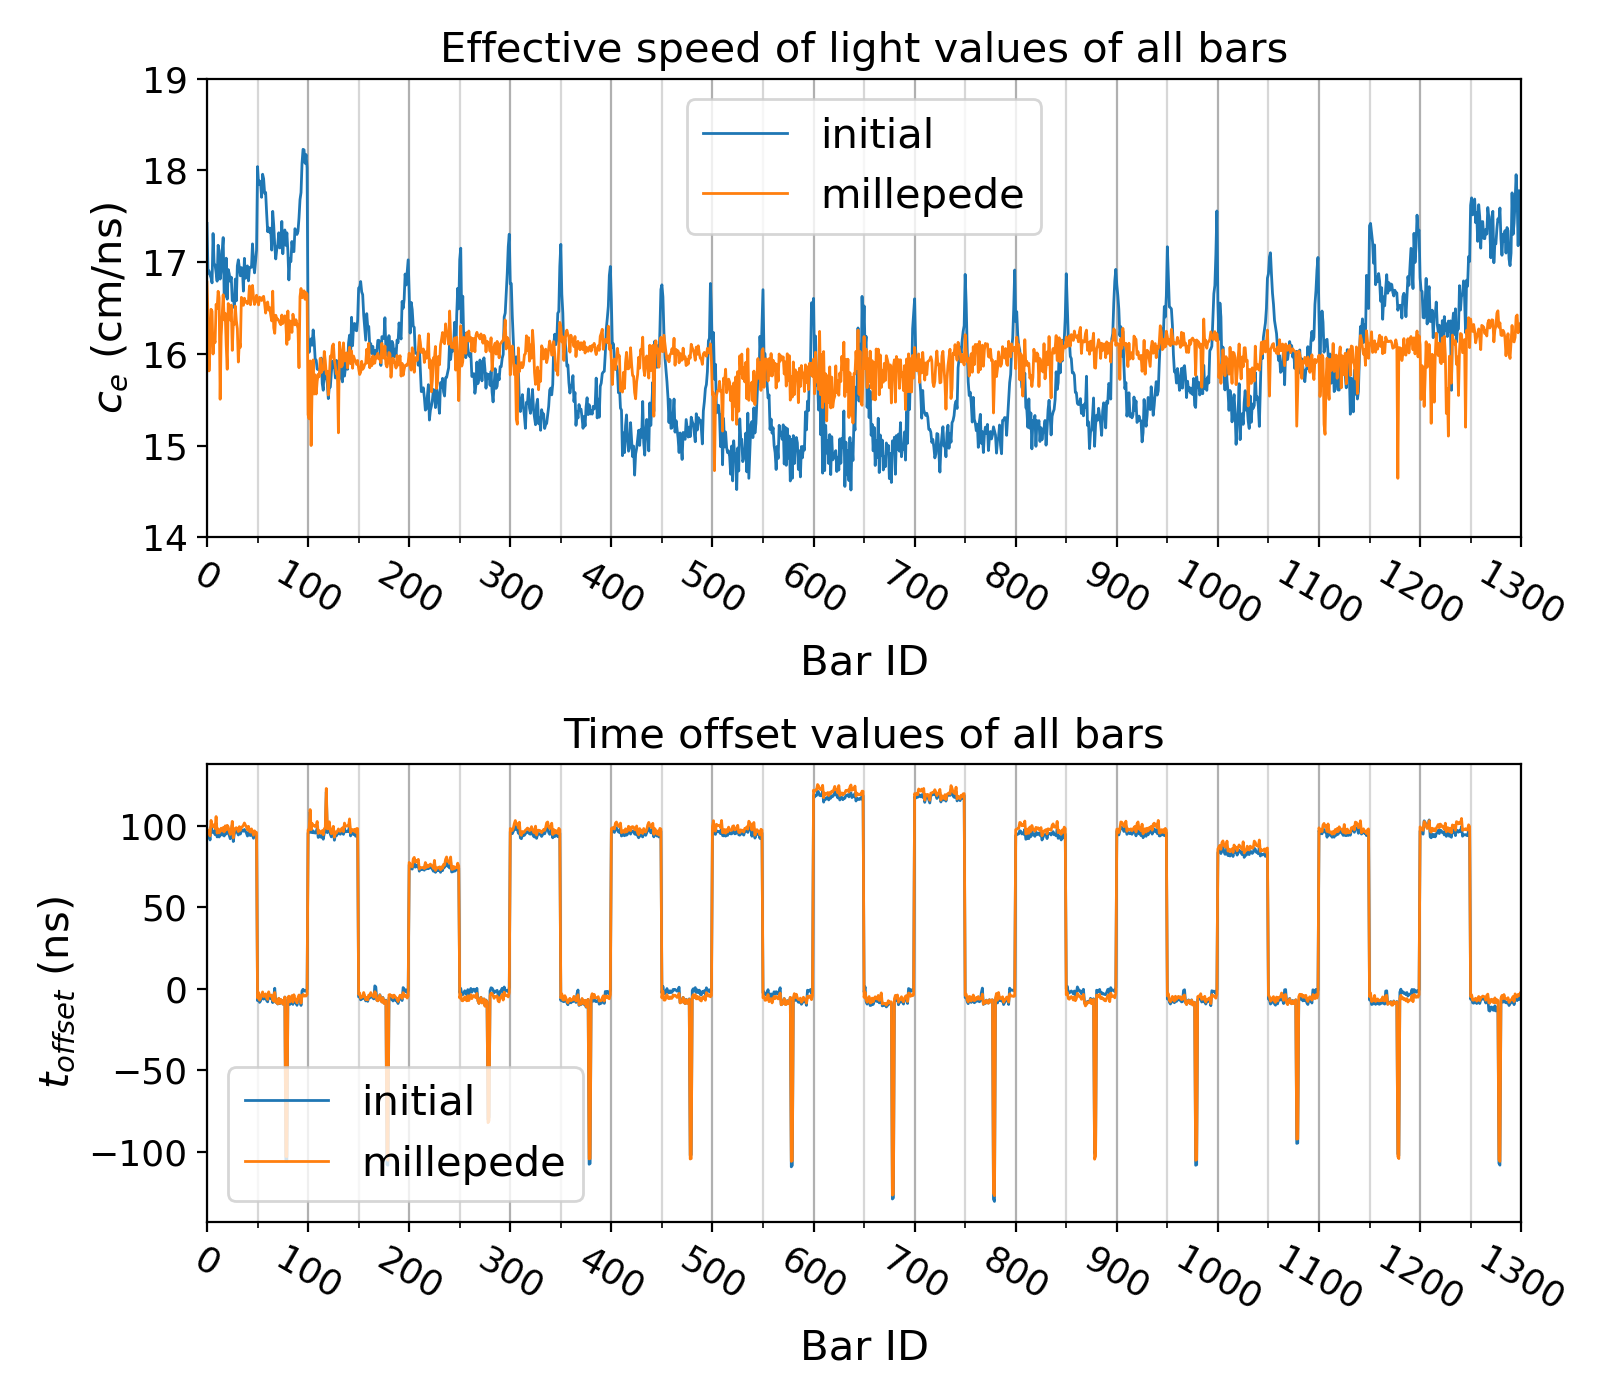
\includegraphics[width=\textwidth]{DPG2026/EffectiveSpeedInitCompare}
				\end{center}
			\end{figure}
		\end{column}
		\begin{column}{0.45 \textwidth}
			\pause
			\textbf{\small Verification through reconstructed muon track}
			\vspace{-1em}
			\begin{figure}
				\begin{center}
					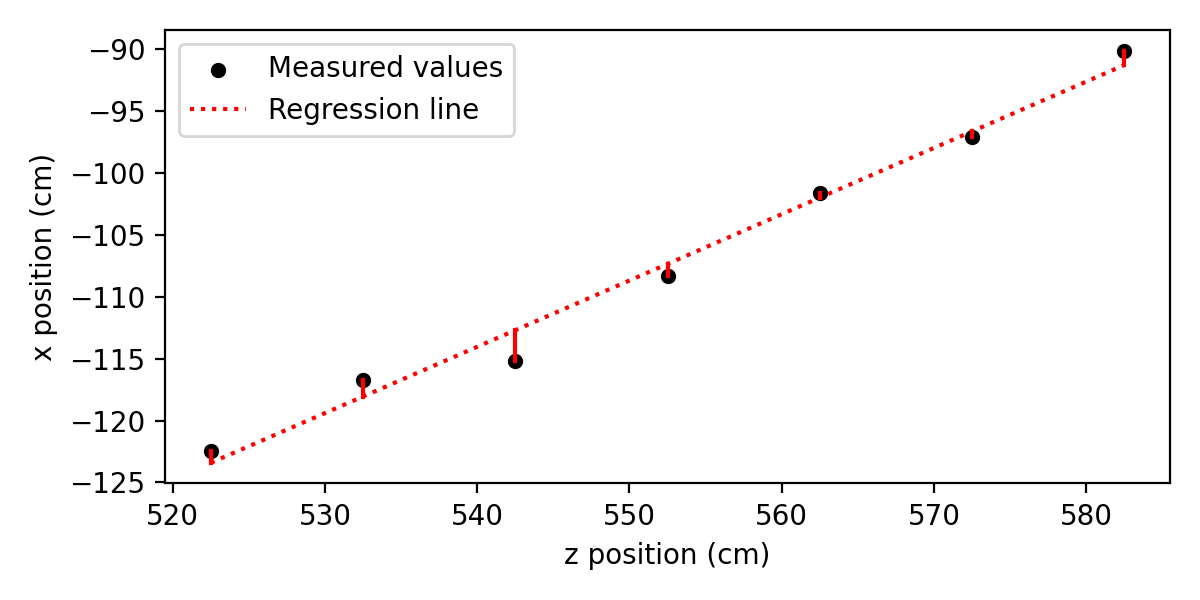
\includegraphics[width=\textwidth]{DPG2026/Residual}
				\end{center}
			\end{figure}
			\vspace{-1.5em}
			{
				\small
				\begin{equation*}
					\text{Residual} = \text{predicted value} - \text{measured value}
				\end{equation*}
			}
			\vspace{-2em}
			\begin{figure}
				\begin{center}
					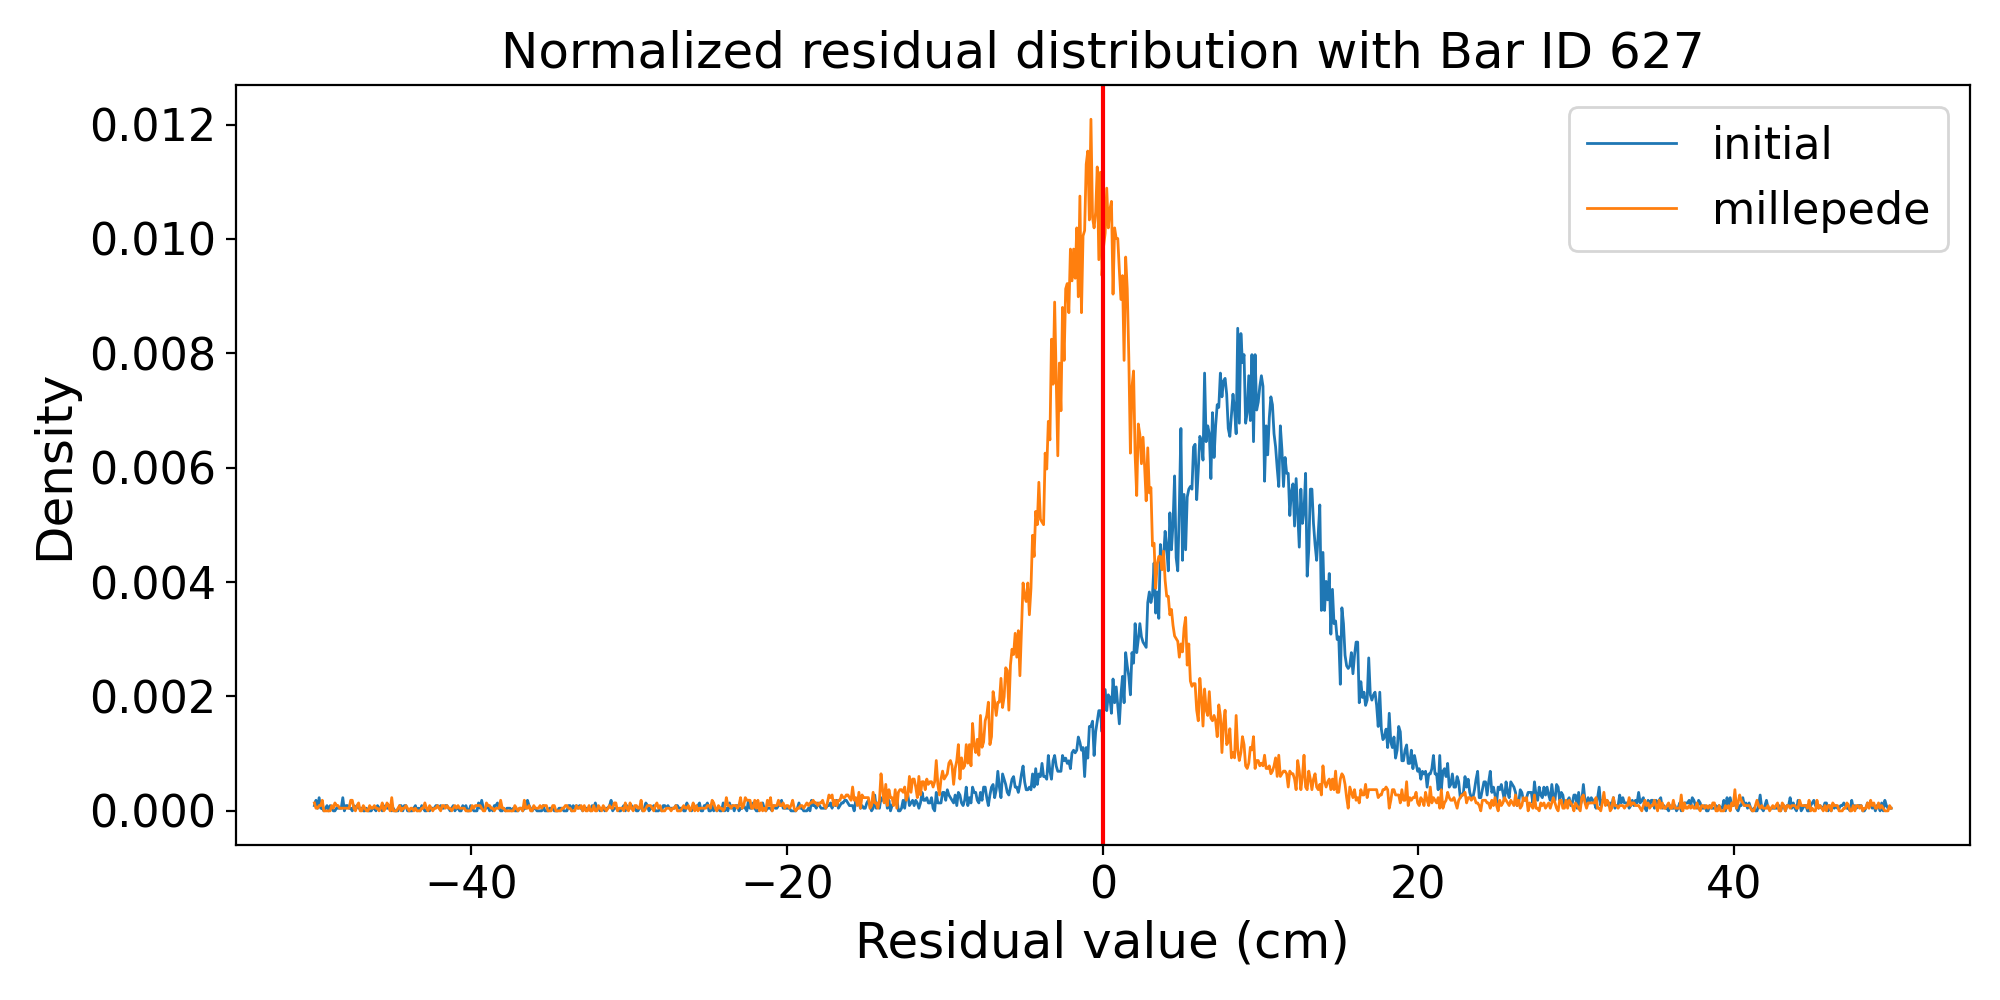
\includegraphics[width=\textwidth]{DPG2026/ResidualSingleBar}
				\end{center}
			\end{figure}
		\end{column}
	\end{columns}

\end{frame}

\begin{frame}[t]{Comparison with the current method}
	\begin{figure}
		\centering
		\begin{tikzpicture}
			\coordinate (TopLeft) at (10, 3);
			\coordinate (BottomRight) at (12, 6);
			\node[anchor=south west,inner sep=0](image) at (0, 0) {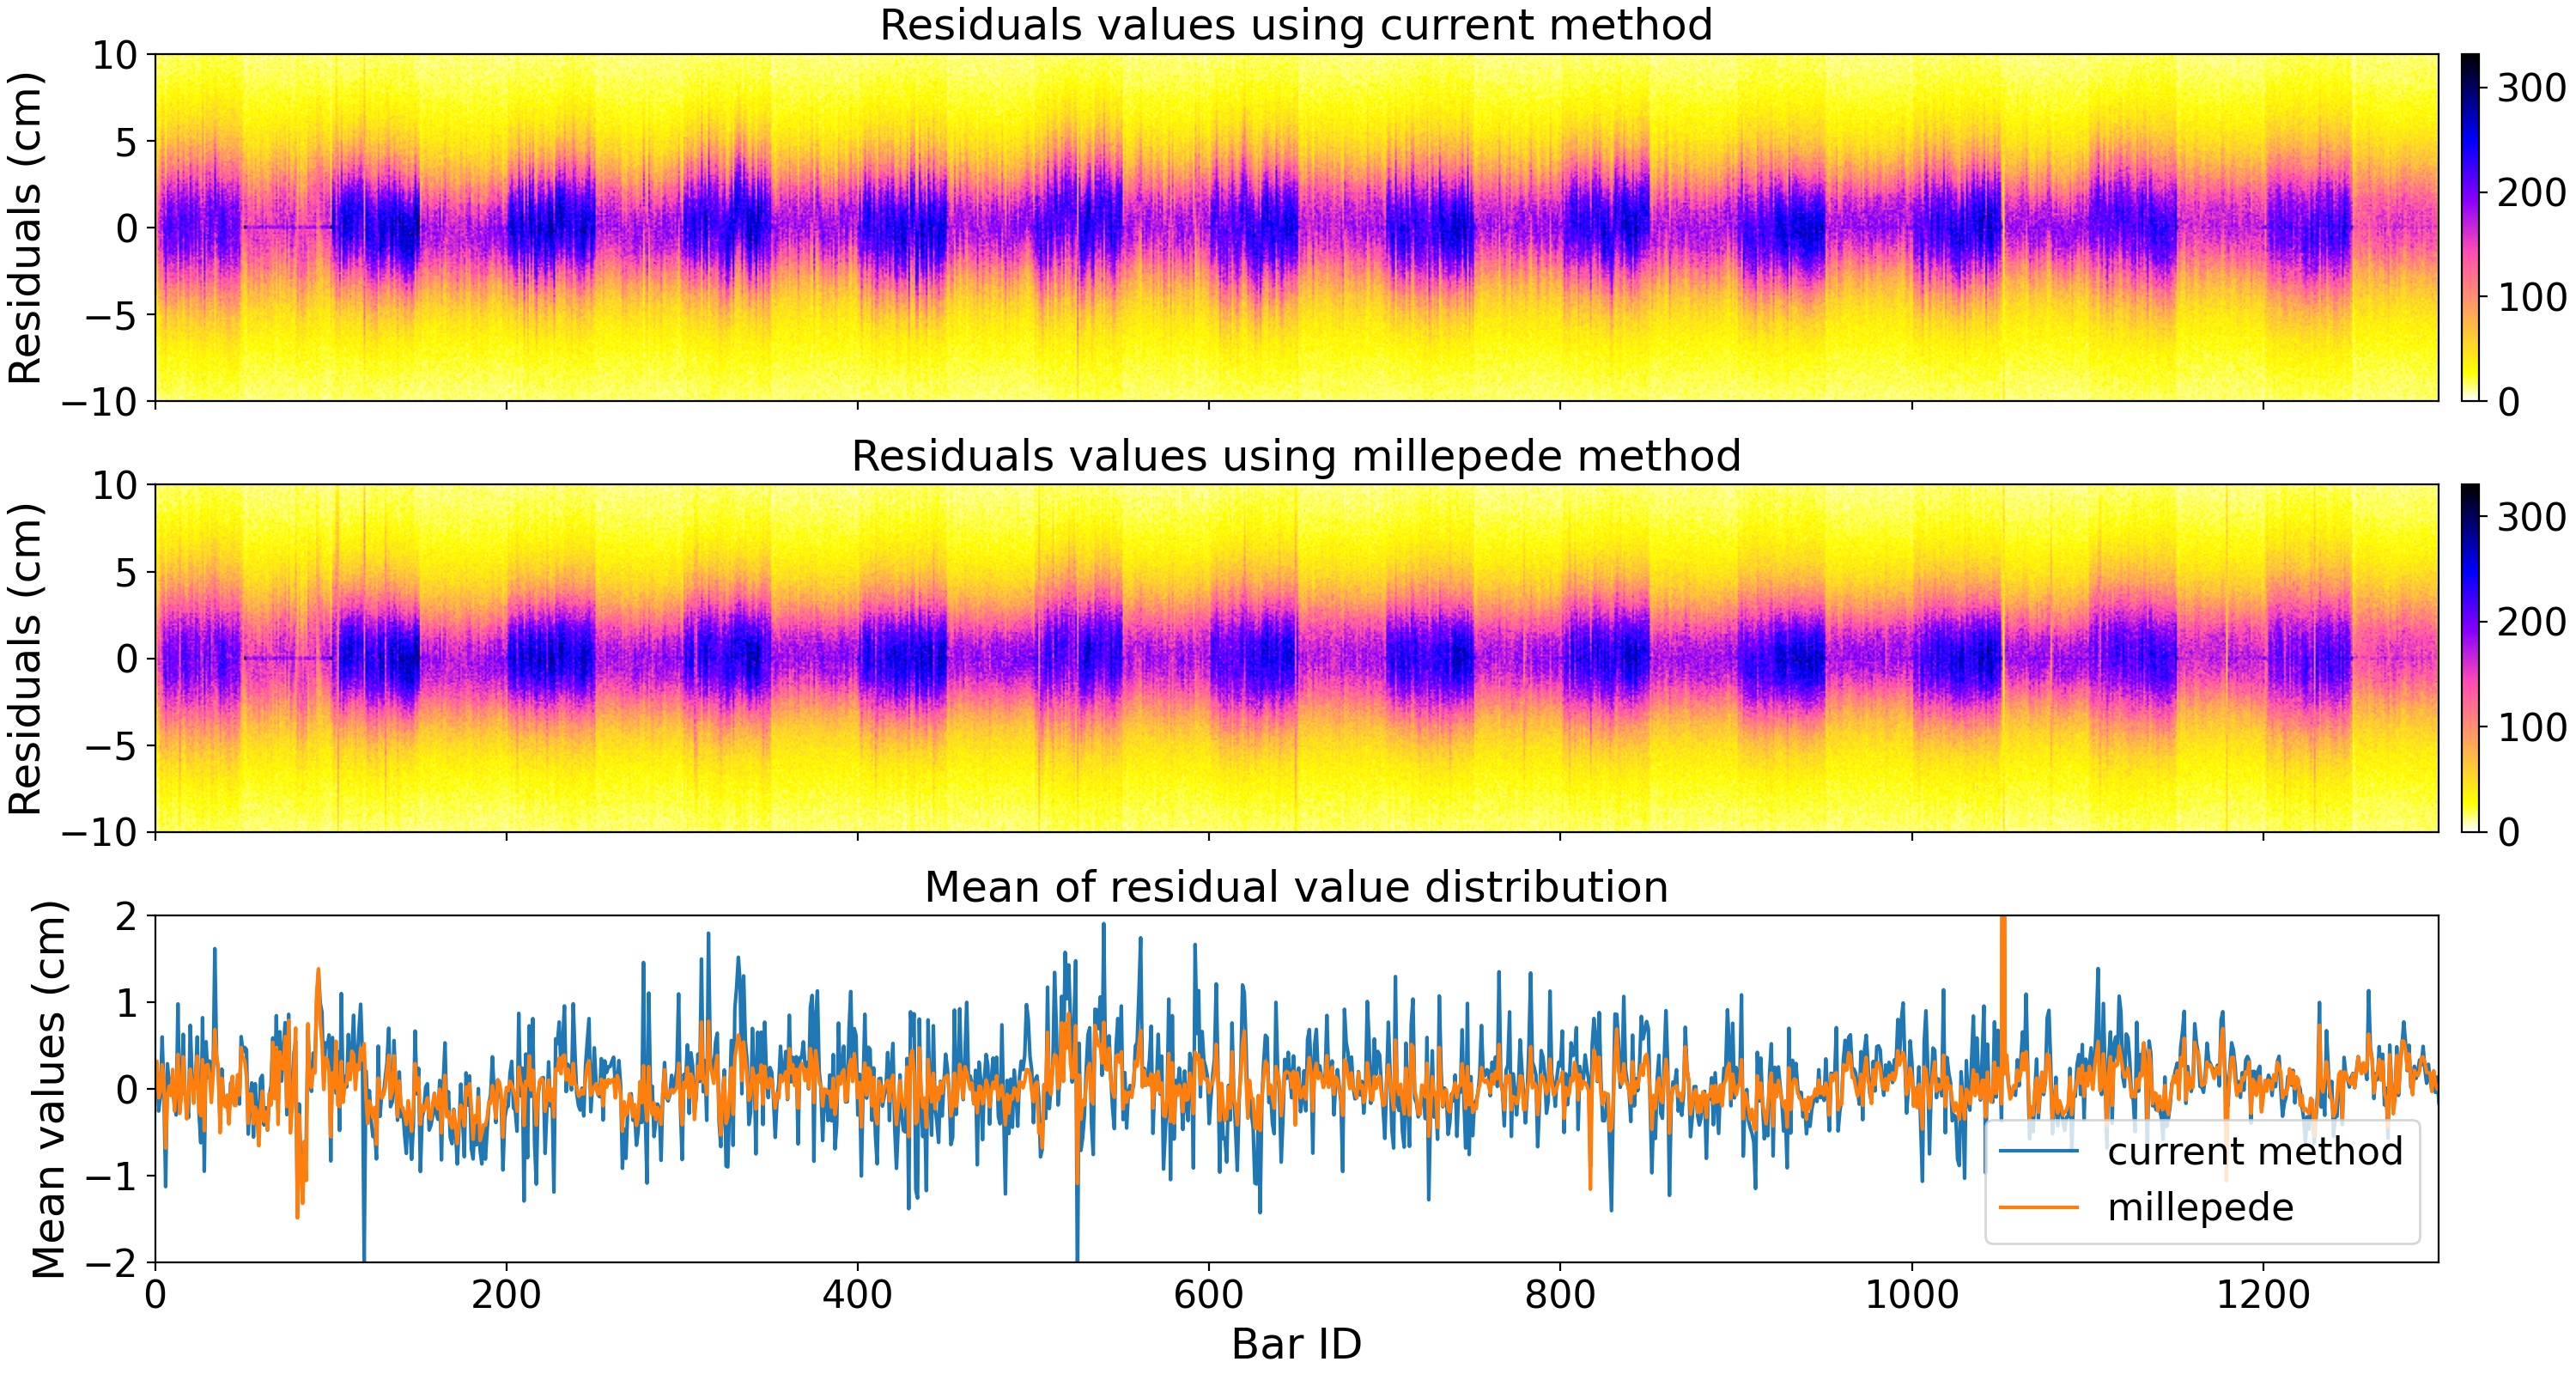
\includegraphics[width=0.9\textwidth]{DPG2026/ResidualCmpCurrent}};
			\draw[red,very thick] (5.5, 3) rectangle (7, 7);
			% \draw (TopLeft) -- (TopLeft |- BootomRight) -- ;
		\end{tikzpicture}
	\end{figure}

\end{frame}

\begin{frame}[t]{Summary and outlook}
	\vspace{-2em}
	\begin{columns}[t]
		\begin{column}{0.45 \textwidth}
			\begin{block}{Summary}
				\begin{itemize}
					\item Millepede algorithm reduces the computation complexity of the calibration processes using cosmic muons.
					\item New method using Millepede algorithm produce less biased results compared to the current method.
				\end{itemize}
			\end{block}

			\begin{exampleblock}{Outlook}
				\begin{itemize}
					\item Implementing the millepede algorithm with modern C++ for a better integration with the current software framework.
					\item Applying millepede algorithm to the energy related parameters as well.
				\end{itemize}
			\end{exampleblock}
		\end{column}
		\begin{column}{0.45 \textwidth}
			\begin{figure}
				\begin{center}
					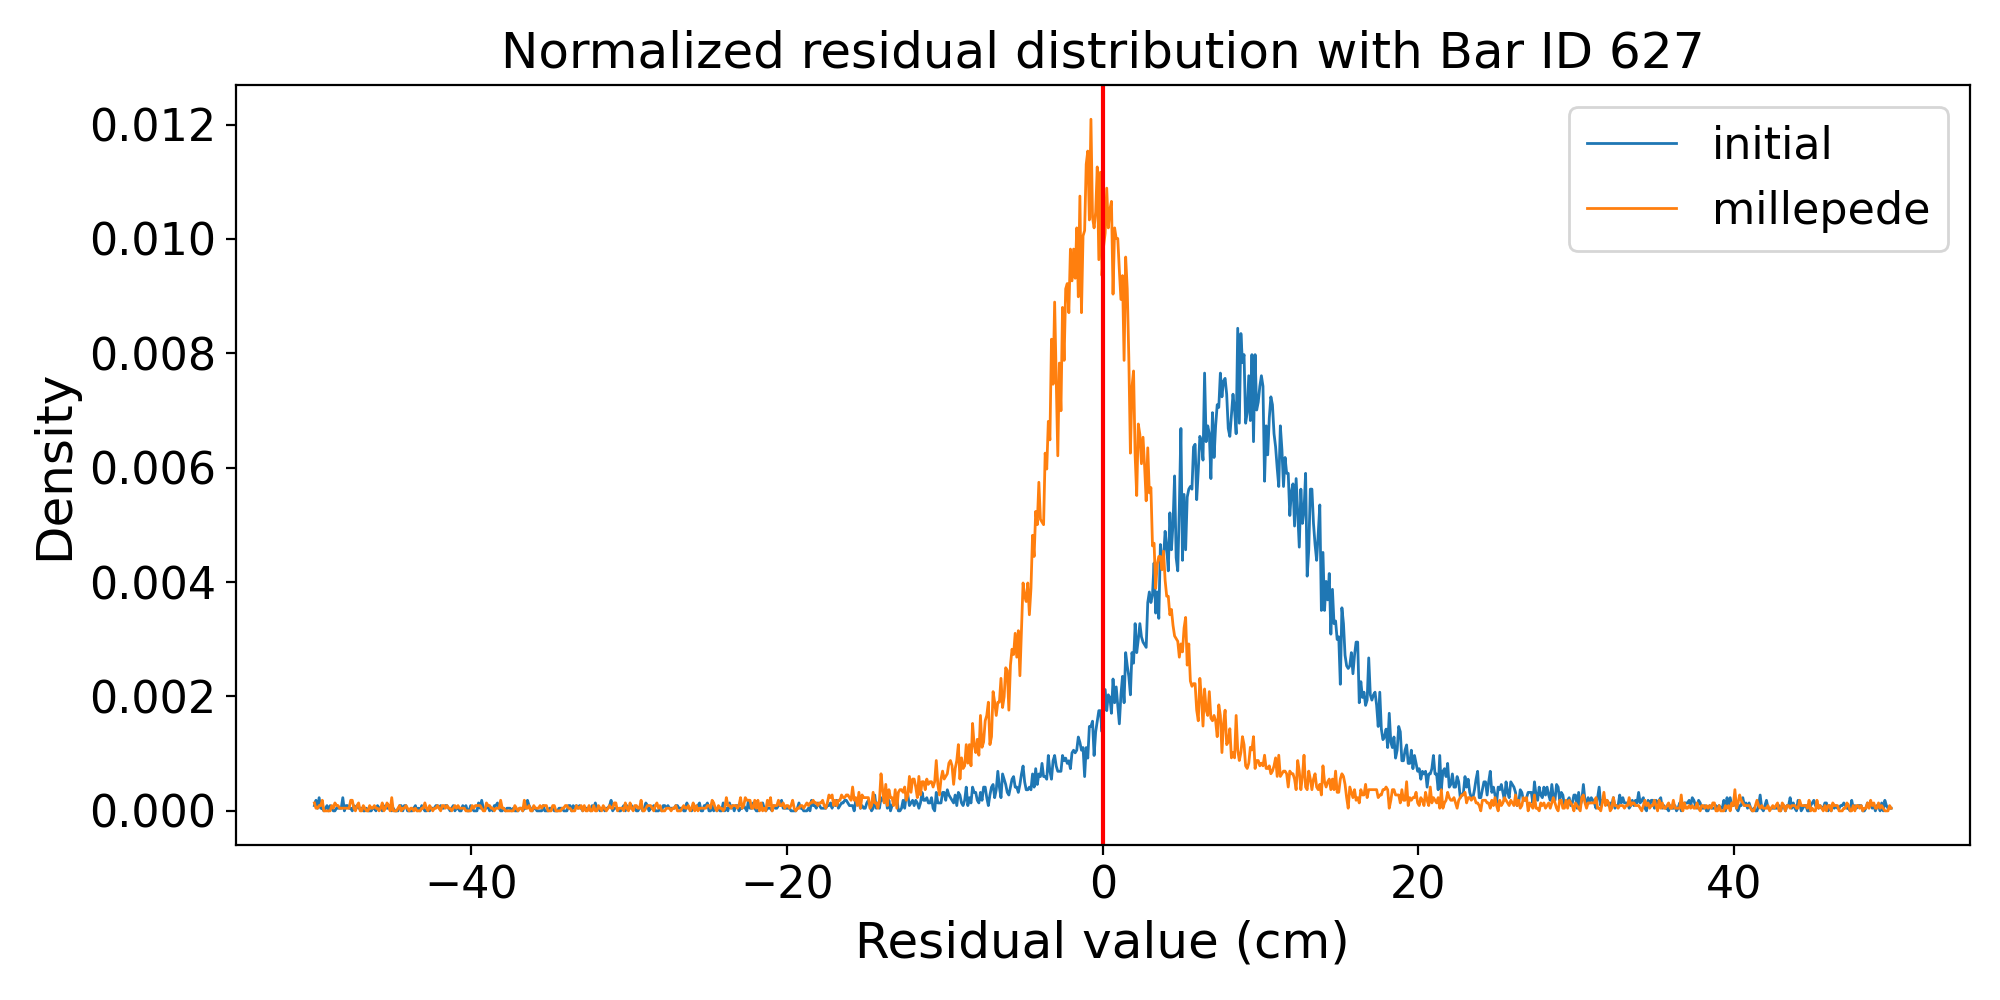
\includegraphics[width=\textwidth]{DPG2026/ResidualSingleBar}
				\end{center}
			\end{figure}
			\vspace{-2em}
			\begin{figure}
				\begin{center}
					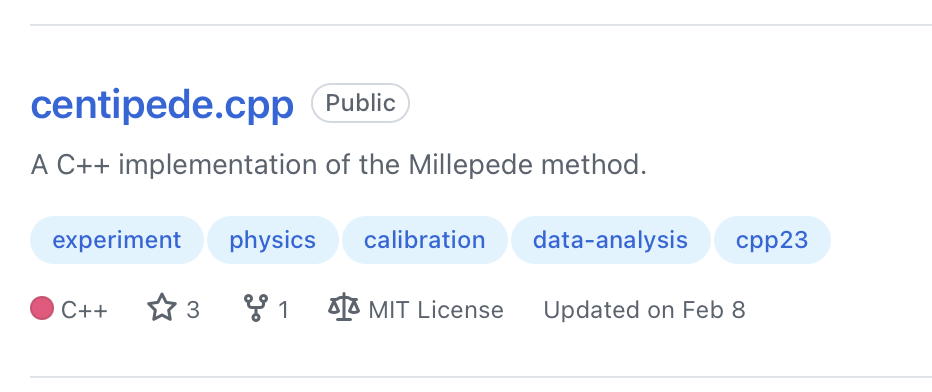
\includegraphics[width=\textwidth]{DPG2026/GithubCentipede}
					\caption*{\scriptsize URL: \url{https://github.com/YanzhaoW/centipede.cpp}}
				\end{center}
			\end{figure}
		\end{column}
	\end{columns}

\end{frame}

\end{document}
